\documentclass[12pt,a4paper]{article}

\usepackage[a4paper,margin=1in]{geometry}
\usepackage{graphicx}
\usepackage{booktabs}
\usepackage{amsmath,amssymb}
\usepackage{float}
\usepackage{hyperref}
\usepackage{xcolor}
\usepackage{listings}
\usepackage{enumitem}
\usepackage{fancyhdr}
\usepackage{longtable}

\hypersetup{colorlinks=true,linkcolor=blue,urlcolor=blue}

\pagestyle{fancy}
\fancyhf{}
\lhead{ICS1512}
\rhead{Machine Learning Algorithms Laboratory}
\cfoot{\thepage}

\lstset{
language=Python,
basicstyle=\ttfamily\small,
numbers=left,
frame=single,
breaklines=true,
showstringspaces=false
}

\begin{document}

\begin{tabular}{|p{4cm}|p{11cm}|}
\hline
Experiment No. & 2 \\ \hline
Experiment Title & Email Spam/Ham Classification using Na\"ive Bayes and KNN\footnotemark\\ \hline
Student Name & Simiyon Vinscent Samuel L \\ \hline
Register Number & 3122247001062 \\ \hline
Faculty & Dr. Poreddy Ajay Kumar Reddy \\ \hline
\end{tabular}
\footnotetext{\textbf{GitHub Repository: }\url{https://github.com/blackscythe123/Machine-Learning-course}}

\section{Objective}
\begin{itemize}[nosep]
\item Build spam classifiers using Na\"ive Bayes and K-Nearest Neighbors (KNN).
\item Compare Gaussian, Multinomial, and Bernoulli Na\"ive Bayes variants.
\item Study the effect of varying $k$ on KNN performance.
\item Compare the KDTree and BallTree neighbor-search algorithms.
\item Optimize KNN using GridSearchCV and RandomizedSearchCV.
\item Evaluate computational (training/prediction) time and theoretical complexity.
\item Evaluate all models using 5-Fold Cross-Validation.
\end{itemize}

\section{Problem Statement}
Given a collection of 4601 emails represented by 57 numeric features derived from word
frequencies, character frequencies, and capital-letter run-length statistics, the task is
to build a \textbf{binary classifier} that labels each email as \textit{spam} (1) or
\textit{ham} (0). Two families of classifiers are studied: probabilistic Na\"ive Bayes
classifiers (Gaussian, Multinomial, Bernoulli) and the instance-based K-Nearest Neighbors
algorithm. Beyond obtaining a well-performing classifier, the aim is to understand
\emph{why} each algorithm behaves the way it does on this dataset, covering accuracy,
precision/recall trade-offs, hyperparameter sensitivity, and computational cost.

\section{Dataset Description}
\begin{longtable}{|p{6cm}|p{8cm}|}
\hline
Dataset Name & Spambase \\ \hline
Dataset Source & UCI Machine Learning Repository / Kaggle
(\url{https://www.kaggle.com/datasets/somesh24/spambase}) \\ \hline
Number of Samples & 4601 \\ \hline
Number of Features & 57 (48 word-frequency, 6 character-frequency, 3 capital-run-length
features) \\ \hline
Number of Classes & 2 (Spam = 1813, 39.40\%; Ham = 2788, 60.60\%) \\ \hline
Missing Values & 0 (verified, no imputation required) \\ \hline
Train-Test Split & 80\% train (3680 samples) / 20\% test (921 samples), stratified on
the class label \\ \hline
\end{longtable}

\section{Exploratory Data Analysis}
\begin{figure}[H]
\centering

\includegraphics[width=\linewidth]{figures/00_eda_summary.png}
\caption{Consolidated exploratory data analysis (12 subplots, single page): (1) class
distribution; (2--7) distributions of the six most class-correlated features, split by
class and clipped at the 95th percentile; (8) correlation heatmap of the ten most
class-correlated features; (9--11) boxplots of the three most discriminating features by
class; (12) scatter of the two most correlated features, coloured by class. Exported at
600 DPI as \texttt{figures/00\_eda\_summary.eps} and reproduced here as PNG.}
\end{figure}

\textbf{Inference (subplot 1, class distribution):} The dataset contains 2788 ham emails
(60.6\%) and 1813 spam emails (39.4\%), a moderate class imbalance rather than a severe
one. Because the imbalance is mild, accuracy remains a reasonably informative metric, but
precision, recall and F1-score are still reported throughout to avoid a misleading
picture, particularly since a spam filter's real-world cost of a false negative (spam
reaching the inbox) differs from that of a false positive (a genuine email marked as
spam). Stratified sampling was therefore used for every train-test split and
cross-validation fold so that both classes are represented proportionally in each
partition.

\textbf{Inference (subplots 2--7, feature distributions):} Spam emails show a visibly
higher density at non-zero values of \texttt{word\_freq\_free}, \texttt{word\_freq\_your},
\texttt{char\_freq\_!} and \texttt{char\_freq\_\$}, while ham emails are heavily
concentrated near zero for these features. \texttt{capital\_run\_length\_average} is also
right-shifted for spam. All features are strongly right-skewed with a long tail of large
values, which is the reason Gaussian Na\"ive Bayes (which assumes normally distributed
features) is expected to under-perform relative to Bernoulli Na\"ive Bayes on this data.

\textbf{Inference (subplot 8, correlation heatmap):} Among all 57 features,
\texttt{word\_freq\_your} (r = 0.383), \texttt{word\_freq\_you} (r = 0.274),
\texttt{word\_freq\_free} (r = 0.263), and the two capital-run-length features
(r $\approx$ 0.22--0.25) show the strongest positive correlation with the spam label.
This matches intuition: spam emails tend to address the reader directly (``you'',
``your''), advertise free offers, and use long runs of capital letters for emphasis. No
pair of features shows extreme multicollinearity ($|r| > 0.9$), so no features were
dropped prior to modelling.

\textbf{Inference (subplots 9--11, boxplots):} The interquartile ranges for
\texttt{word\_freq\_free}, \texttt{word\_freq\_your} and the character-frequency features
are consistently higher and wider for the spam class, which makes them strong
discriminating features. Ham emails have near-zero medians for almost every feature
shown, which explains why simple thresholding on a handful of features (as Bernoulli NB
effectively does after binarization) already achieves strong separation.

\section{Data Preprocessing}
\begin{itemize}
\item \textbf{Missing values:} The dataset was checked with \texttt{isnull().sum()} and
confirmed to contain zero missing entries, so no imputation was necessary.
\item \textbf{Encoding:} All 57 features are numeric (frequencies and run-length
statistics), so no categorical encoding was required.
\item \textbf{Feature scaling:} Two parallel versions of the feature matrix were
prepared:
  \begin{itemize}
  \item A \textbf{standardized} version (\texttt{StandardScaler}, zero mean / unit
  variance fitted on the training set only) used for \textbf{Gaussian NB} and
  \textbf{KNN}, since both algorithms are scale-sensitive.
  \item The \textbf{original non-negative} version used for \textbf{Multinomial NB} and
  \textbf{Bernoulli NB}, since these variants require non-negative (count-like) input
  and standardization would introduce negative values that violate their assumptions.
  \end{itemize}
\item \textbf{Train-test split:} An 80/20 stratified split (\texttt{random\_state=42})
was used, giving 3680 training and 921 test samples with class proportions preserved.
\item \textbf{Feature engineering:} No additional feature engineering was performed; the
57 provided attributes were used as-is, consistent with the standard Spambase benchmark.
\end{itemize}

\section{Machine Learning Algorithm}

\subsection*{Na\"ive Bayes}
Na\"ive Bayes is a probabilistic classifier based on Bayes' theorem with a conditional
independence assumption between features given the class:
\[
P(C \mid X) = \frac{P(X \mid C)\,P(C)}{P(X)}, \qquad
P(X\mid C) = \prod_{i=1}^{d} P(x_i \mid C)
\]
Three variants differ in how $P(x_i \mid C)$ is modelled:
\begin{itemize}
\item \textbf{Gaussian NB} assumes $x_i \mid C \sim \mathcal{N}(\mu_C, \sigma_C^2)$,
appropriate for continuous, roughly bell-shaped features.
\item \textbf{Multinomial NB} models $x_i$ as counts drawn from a multinomial
distribution, naturally suited to word/token counts.
\item \textbf{Bernoulli NB} binarizes each feature ($x_i > 0 \Rightarrow 1$, else $0$)
and models presence/absence of a term, explicitly penalizing the \emph{non-occurrence}
of a feature as well as rewarding its occurrence.
\end{itemize}
\textbf{Advantages:} Extremely fast to train (single pass, closed-form parameter
estimates), works well with high-dimensional data, requires little training data.
\textbf{Limitations:} The conditional-independence assumption rarely holds exactly;
Gaussian NB is sensitive to non-normal feature distributions (as seen in this dataset).

\subsection*{K-Nearest Neighbors (KNN)}
KNN is a lazy, instance-based learner. To classify a query point $x$, it finds the $k$
training points closest to $x$ (by a distance metric such as Euclidean or Manhattan
distance) and assigns the majority class among them:
\[
\hat{y} = \operatorname*{arg\,max}_{c} \sum_{i \in N_k(x)} \mathbb{1}(y_i = c)
\]
where $N_k(x)$ is the set of $k$ nearest neighbors, optionally weighted by inverse
distance (\texttt{weights='distance'}). Neighbor search can be performed by
\textbf{brute force} ($O(nd)$ per query), or accelerated with spatial index structures:
\begin{itemize}
\item \textbf{KDTree} -- partitions the feature space along axis-aligned hyperplanes;
efficient in low-to-moderate dimensions.
\item \textbf{BallTree} -- partitions data into nested hyperspheres; more robust in
higher dimensions than KDTree.
\end{itemize}
\textbf{Advantages:} No training phase, naturally handles multi-modal class boundaries,
simple to understand. \textbf{Limitations:} Prediction is expensive at scale, sensitive
to feature scaling and irrelevant features, and both KDTree and BallTree degrade toward
brute-force performance as dimensionality increases (the ``curse of dimensionality''),
a relevant concern here since $d = 57$.

\section{Experimental Setup}
\begin{tabular}{ll}
\toprule
Python Version & 3.12.3 \\
Scikit-Learn Version & 1.8.0 \\
IDE & Jupyter Notebook \\
Operating System & Windows 11 \\
Hardware & Intel Core Ultra 9, NVIDIA RTX 5060 \\
\bottomrule
\end{tabular}

\section{Hyperparameter Selection}

\begin{tabular}{ll}
\toprule
Parameter & Search Space \\
\midrule
KNN -- n\_neighbors (Grid) & $\{1,3,5,7,9,11,13,15\}$ \\
KNN -- n\_neighbors (Random) & $\{1,2,\dots,25\}$ \\
KNN -- weights & \{uniform, distance\} \\
KNN -- algorithm & \{kd\_tree, ball\_tree\} \\
KNN -- metric & \{euclidean, manhattan\} \\
Cross-validation & 5-fold stratified (\texttt{StratifiedKFold}) \\
RandomizedSearchCV iterations & 25 (of 128 possible combinations) \\
\bottomrule
\end{tabular}

\bigskip
\begin{tabular}{lll}
\toprule
Parameter & GridSearchCV & RandomizedSearchCV \\
\midrule
Best $k$ & 9 & 8 \\
Metric & manhattan & manhattan \\
Weights & distance & distance \\
Algorithm & kd\_tree & ball\_tree \\
Best CV Accuracy & 0.9253 & 0.9255 \\
Execution Time (s) & 58.52 & 23.77 \\
\bottomrule
\end{tabular}

\section{Results}

\subsection*{Na\"ive Bayes Comparison (Test Set)}
\begin{tabular}{lccc}
\toprule
Metric & Gaussian & Multinomial & Bernoulli \\
\midrule
Accuracy  & 0.8328 & 0.7763 & \textbf{0.8762} \\
Precision & 0.7146 & 0.7199 & \textbf{0.8716} \\
Recall    & \textbf{0.9587} & 0.7080 & 0.8044 \\
F1-Score  & 0.8188 & 0.7139 & \textbf{0.8367} \\
ROC-AUC   & 0.9376 & 0.8248 & \textbf{0.9496} \\
\bottomrule
\end{tabular}

\subsection*{KNN: Accuracy vs. $k$ (Test Set, uniform weights, Euclidean distance)}
\begin{tabular}{lcccc}
\toprule
$k$ & Accuracy & Precision & Recall & F1-Score \\
\midrule
1  & 0.8990 & 0.8792 & 0.8623 & 0.8707 \\
3  & 0.8979 & 0.8726 & 0.8678 & 0.8702 \\
5  & 0.9077 & 0.8861 & 0.8788 & 0.8824 \\
7  & 0.9088 & 0.8930 & 0.8733 & 0.8830 \\
9  & 0.9088 & 0.8930 & 0.8733 & 0.8830 \\
11 & \textbf{0.9099} & \textbf{0.9000} & 0.8678 & \textbf{0.8836} \\
\bottomrule
\end{tabular}

\subsection*{KDTree vs. BallTree ($k=11$, uniform weights)}
\begin{tabular}{lccc}
\toprule
Metric & KDTree & BallTree \\
\midrule
Accuracy & 0.9099 & 0.9099 \\
Training Time (s) & 0.0167 & \textbf{0.0115} \\
Prediction Time (s) & 0.2659 & \textbf{0.2506} \\
\bottomrule
\end{tabular}

\subsection*{Tuned Model Performance (Test Set)}
\begin{tabular}{lc}
\toprule
Metric & Value (Best KNN: $k=9$, distance, manhattan, kd\_tree)\\
\midrule
Accuracy & 0.9207 \\
Precision & 0.9421 \\
Recall & 0.8512 \\
F1-score & 0.8944 \\
ROC-AUC & 0.9712 \\
\bottomrule
\end{tabular}

\subsection*{5-Fold Cross-Validation Results (Training Set)}
\begin{tabular}{lcc}
\toprule
Fold & Bernoulli Na\"ive Bayes & Tuned KNN \\
\midrule
1 & 0.9063 & 0.9389 \\
2 & 0.8913 & 0.9280 \\
3 & 0.8723 & 0.9253 \\
4 & 0.8682 & 0.9266 \\
5 & 0.8981 & 0.9076 \\
\midrule
\textbf{Average} & \textbf{0.8872 $\pm$ 0.0147} & \textbf{0.9253 $\pm$ 0.0101} \\
\bottomrule
\end{tabular}

\subsection*{Theoretical Time Complexity}
\begin{tabular}{lll}
\toprule
Algorithm & Training & Prediction \\
\midrule
Na\"ive Bayes & $O(nd)$ & $O(d)$ \\
KNN (Brute) & $O(1)$ & $O(nd)$ \\
KDTree & $O(n\log n)$ & $O(\log n)_{avg}$ \\
BallTree & $O(n\log n)$ & $O(\log n)_{avg}$ \\
\bottomrule
\end{tabular}
\vspace{2mm}
\textit{Here $n = 3680$ (training samples) and $d = 57$ (features).}

\subsection*{Experimental Time Analysis}
\begin{tabular}{lcc}
\toprule
Algorithm & Training Time (s) & Prediction Time (s, full test set) \\
\midrule
Gaussian NB & 0.00589 & 0.00194 \\
Multinomial NB & \textbf{0.00277} & \textbf{0.00043} \\
Bernoulli NB & 0.00527 & 0.00143 \\
Tuned KNN (kd\_tree) & 0.01600 & 0.28618 \\
\bottomrule
\end{tabular}

\subsection*{Additional Task: Distance Metric Comparison ($k=9$, uniform weights)}
\begin{tabular}{lcccc}
\toprule
Metric & Accuracy & Precision & Recall & F1-Score \\
\midrule
Euclidean & \textbf{0.9088} & 0.8930 & \textbf{0.8733} & \textbf{0.8830} \\
Manhattan & 0.9034 & \textbf{0.9335} & 0.8127 & 0.8689 \\
\bottomrule
\end{tabular}

\subsection*{Additional Task: Weighted KNN Comparison ($k=9$)}
\begin{tabular}{lcccc}
\toprule
Weights & Accuracy & Precision & Recall & F1-Score \\
\midrule
Uniform  & 0.9088 & 0.8930 & 0.8733 & 0.8830 \\
Distance & \textbf{0.9164} & 0.8972 & \textbf{0.8898} & \textbf{0.8935} \\
\bottomrule
\end{tabular}

\subsection*{Additional Task: Train-Test Split Sensitivity}
\begin{tabular}{lccc}
\toprule
Split & Test Accuracy (Bernoulli NB) & Test Accuracy (Tuned KNN) \\
\midrule
70/30 & 0.8870 & \textbf{0.9312} \\
80/20 & 0.8762 & 0.9207 \\
90/10 & 0.8785 & 0.9067 \\
\bottomrule
\end{tabular}

\section{Result Visualization}

\begin{figure}[H]
\centering
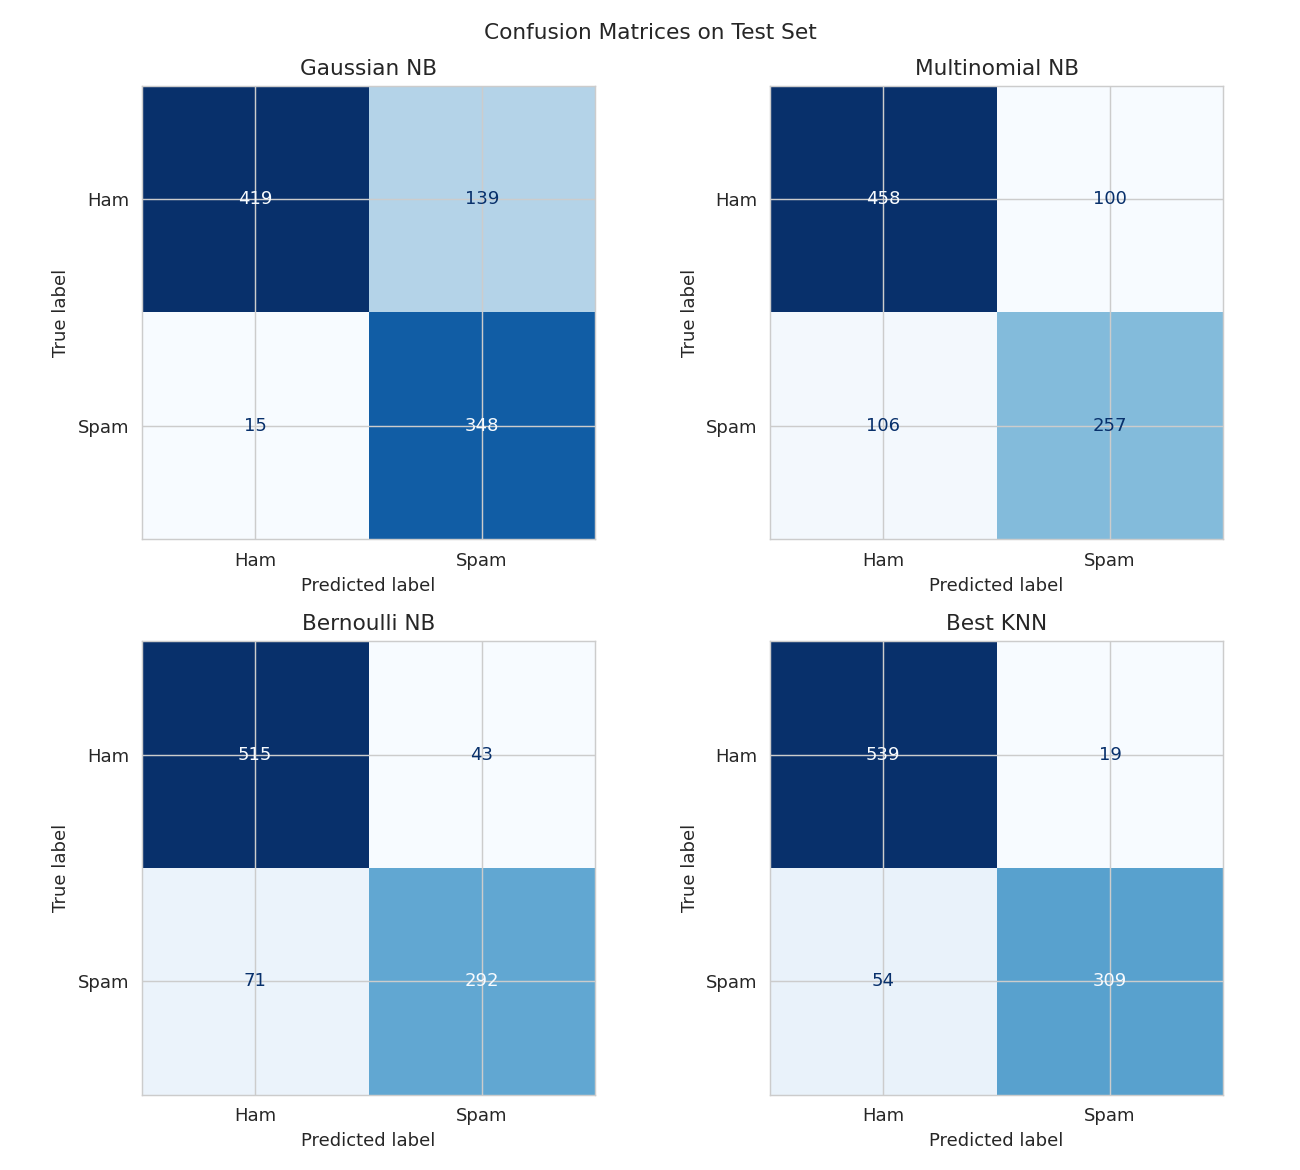
\includegraphics[width=0.95\linewidth]{figures/05_confusion_matrices.png}
\caption{Confusion matrices for all four classifiers on the test set.}
\end{figure}
\textbf{Inference:} Gaussian NB has the fewest false negatives (missed spam) but the most
false positives (ham wrongly marked spam), consistent with its high recall / low
precision profile. Bernoulli NB and the tuned KNN show the most balanced confusion
matrices, with KNN achieving the fewest total misclassifications (73 of 921 test
samples).

\begin{figure}[H]
\centering
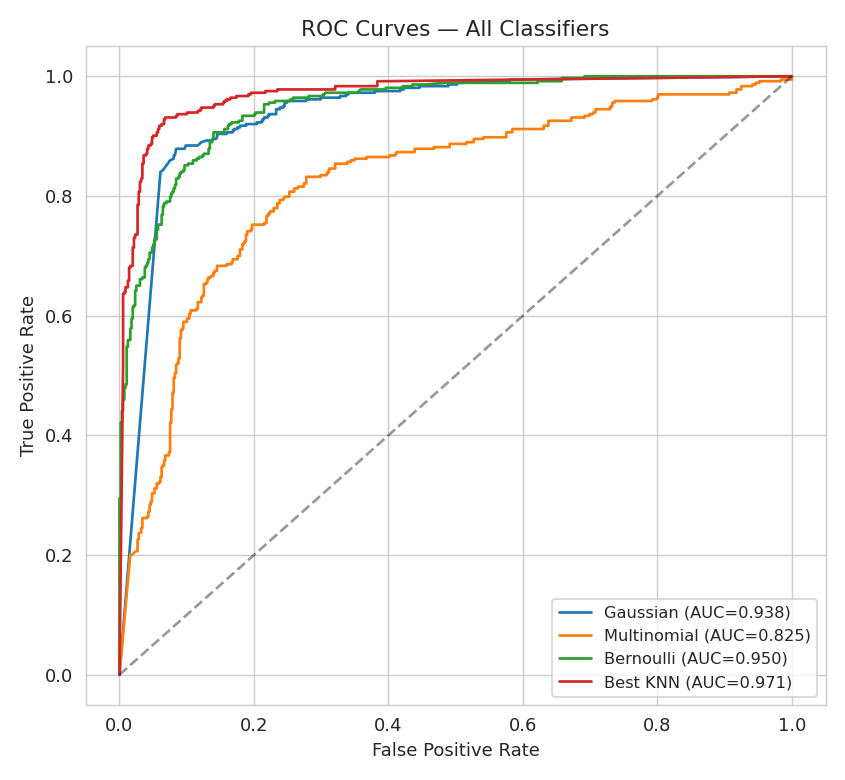
\includegraphics[width=0.7\linewidth]{figures/06_roc_curves.png}
\caption{ROC curves for all classifiers.}
\end{figure}
\textbf{Inference:} The tuned KNN model achieves the highest AUC (0.971), followed
closely by Bernoulli NB (0.950) and Gaussian NB (0.938); Multinomial NB trails with an
AUC of 0.825. All curves lie well above the diagonal, confirming that every classifier
has genuine discriminative power over random guessing.

\begin{figure}[H]
\centering
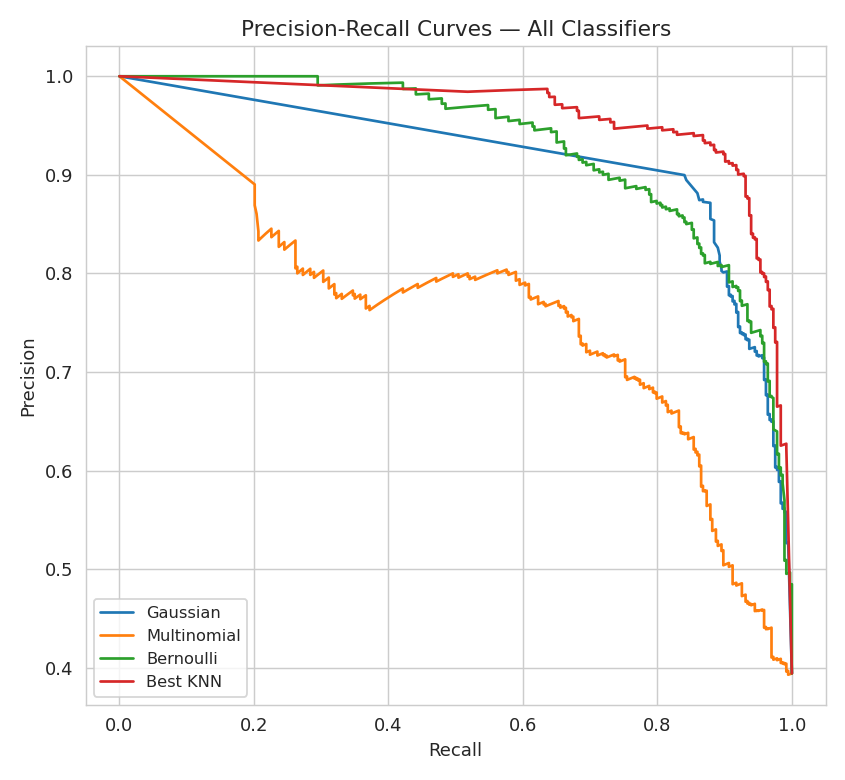
\includegraphics[width=0.7\linewidth]{figures/07_pr_curves.png}
\caption{Precision-Recall curves for all classifiers.}
\end{figure}
\textbf{Inference:} Because spam is the minority class, the PR curve is a stricter test
than ROC. KNN and Bernoulli NB maintain high precision across most of the recall range,
while Gaussian NB's precision drops sharply as recall approaches 1; it achieves high
recall only by aggressively over-predicting the spam class.

\begin{figure}[H]
\centering
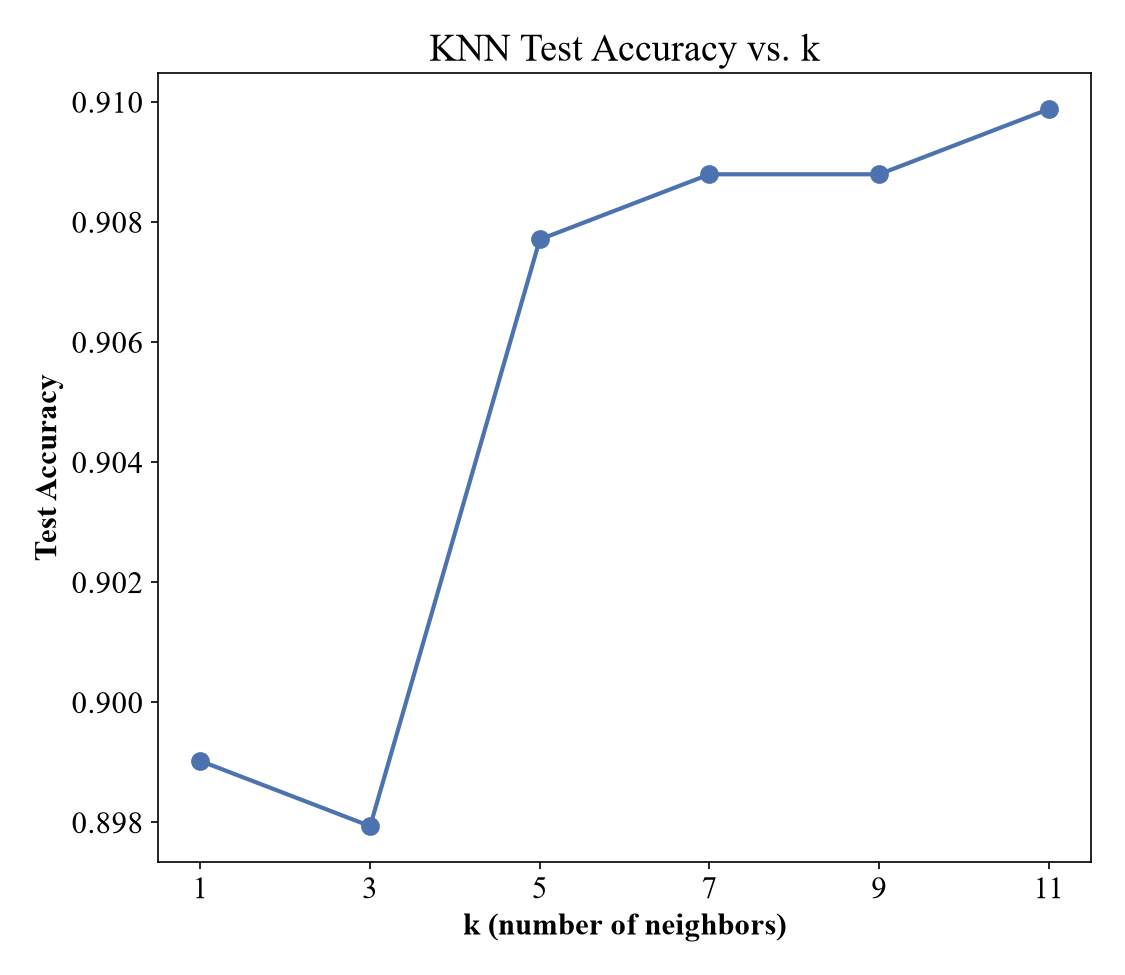
\includegraphics[width=0.6\linewidth]{figures/08_accuracy_vs_k.png}
\caption{KNN test accuracy as a function of $k$.}
\end{figure}
\textbf{Inference:} Accuracy rises from $k=1$ to around $k=7$--$11$ and then plateaus,
indicating that very small $k$ values (especially $k=1$) are noisier / more prone to
overfitting individual training points, while accuracy stabilizes once enough neighbors
are averaged to smooth out noise, without yet showing underfitting.

\begin{figure}[H]
\centering
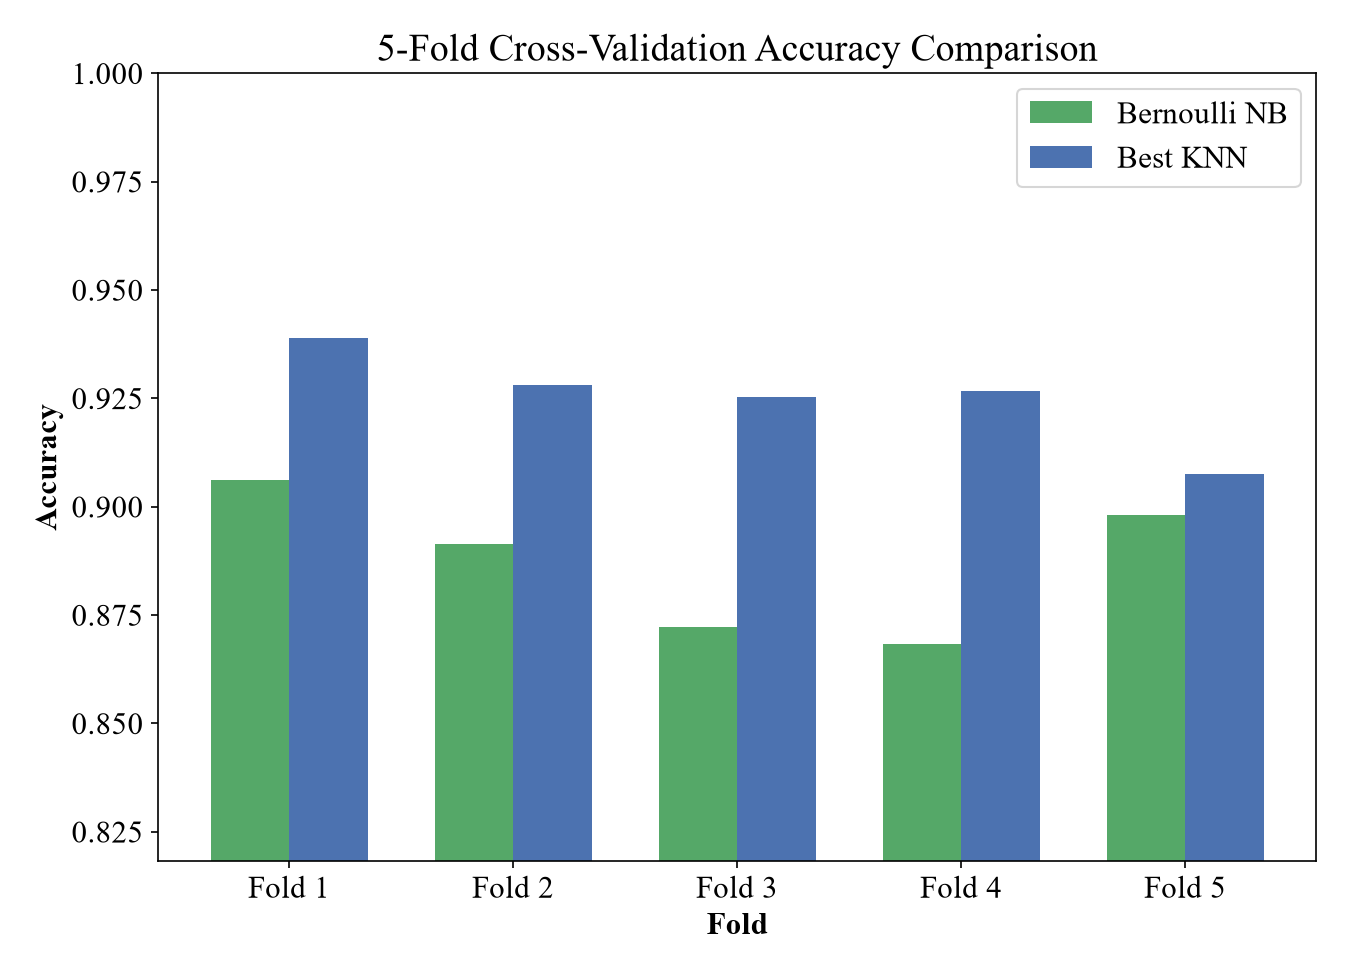
\includegraphics[width=0.65\linewidth]{figures/09_cv_accuracy.png}
\caption{5-fold cross-validation accuracy: Bernoulli NB vs. tuned KNN.}
\end{figure}
\textbf{Inference:} The tuned KNN outperforms Bernoulli NB in every single fold, by a
consistent margin of roughly 3--5 percentage points, so its advantage on the held-out
test set is not a one-off artifact of a single split.

\begin{figure}[H]
\centering
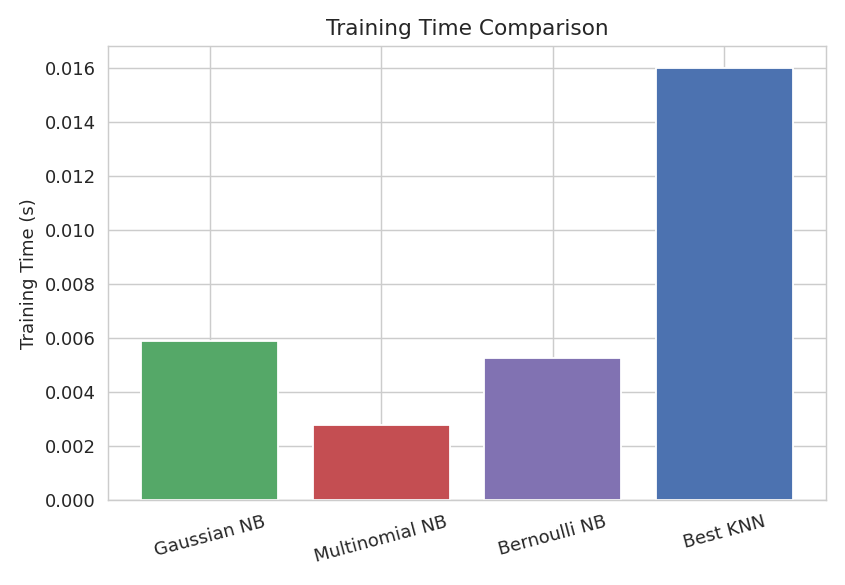
\includegraphics[width=0.6\linewidth]{figures/10_training_time.png}
\caption{Training time comparison across all four classifiers.}
\end{figure}
\textbf{Inference:} All Na\"ive Bayes variants train in under 6 milliseconds since they
only compute closed-form summary statistics. KNN's ``training'' time (here, building the
KD-tree index) is also small (16 ms) since it does no real learning, confirming the
$O(1)$/$O(n\log n)$ theoretical expectation.

\begin{figure}[H]
\centering
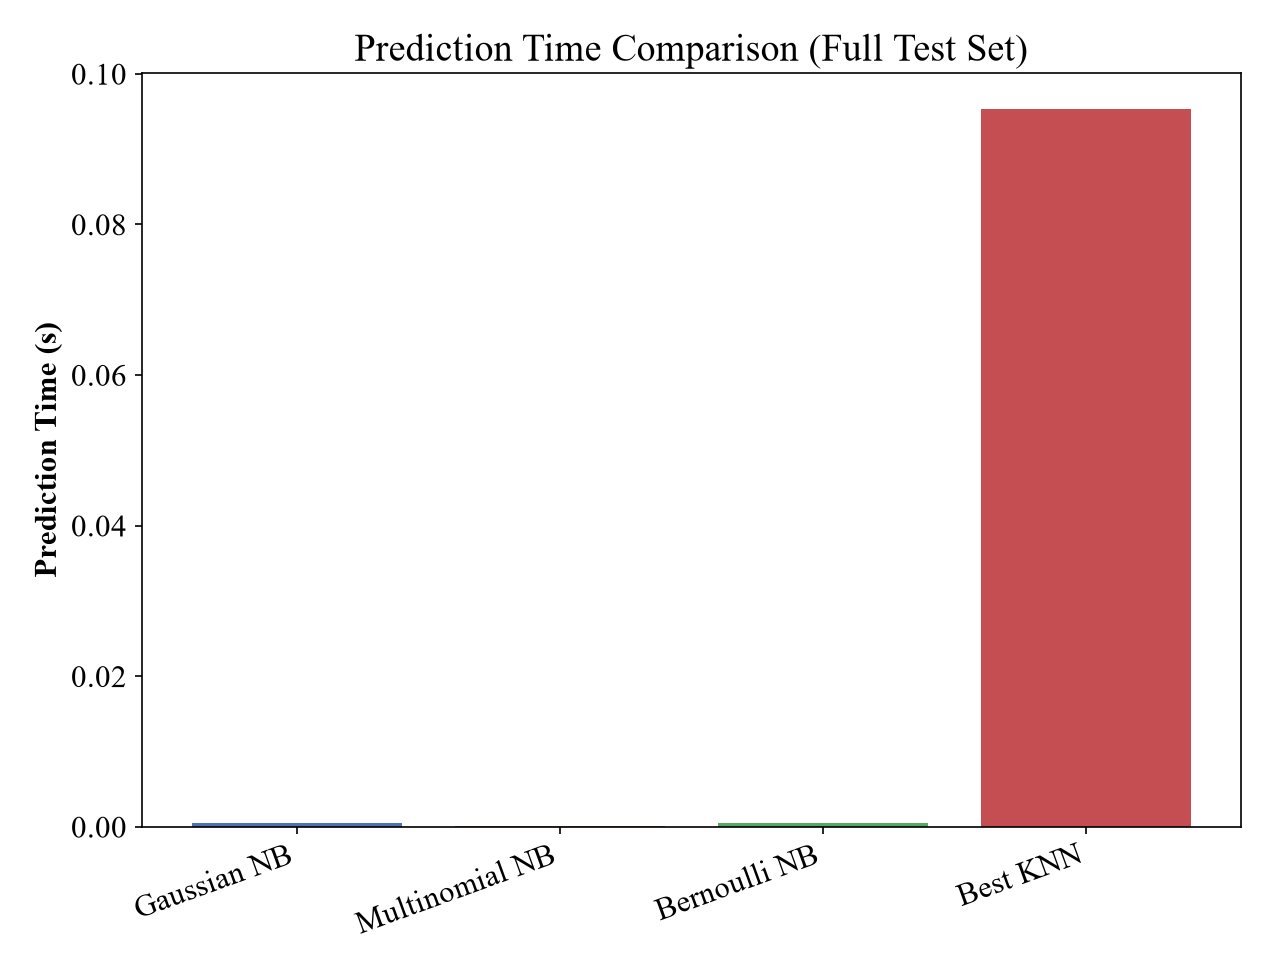
\includegraphics[width=0.6\linewidth]{figures/11_prediction_time.png}
\caption{Prediction time comparison (full 921-sample test set).}
\end{figure}
\textbf{Inference:} KNN prediction is roughly 150--600$\times$ slower than any Naive
Bayes variant, since every query requires a nearest-neighbor search across the training
set. This is the clearest practical illustration of the $O(nd)$/$O(\log n)_{avg}$ vs.
$O(d)$ complexity gap noted in the theoretical table.

\begin{figure}[H]
\centering
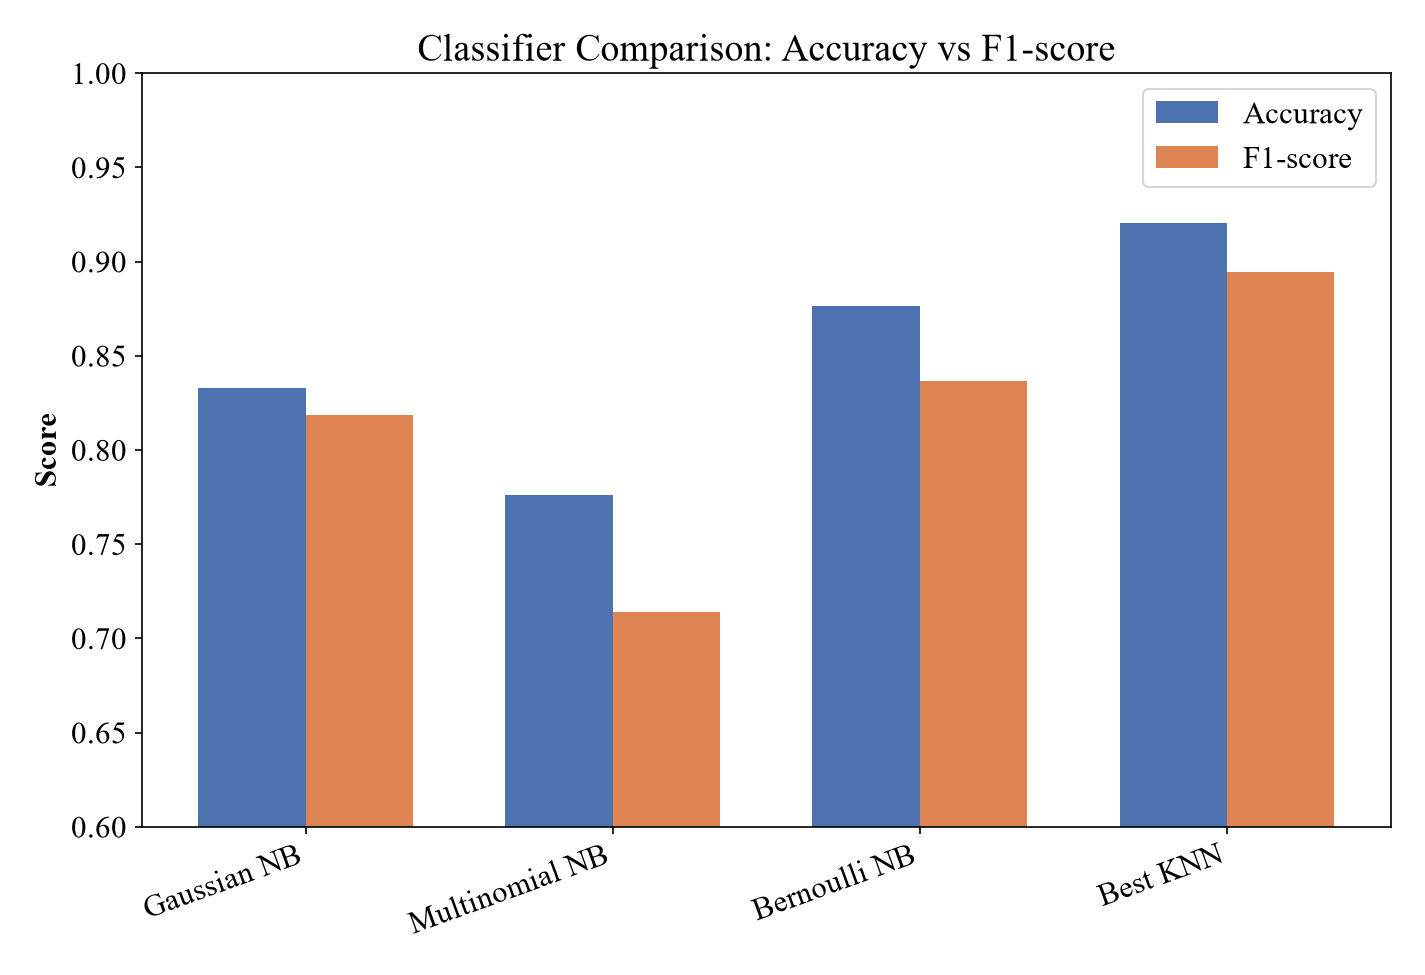
\includegraphics[width=0.65\linewidth]{figures/12_classifier_comparison.png}
\caption{Overall Accuracy and F1-score comparison across all classifiers.}
\end{figure}
\textbf{Inference:} The tuned KNN is the best all-round performer (highest accuracy and
F1), Bernoulli NB is a close, much faster runner-up, and Multinomial NB is the weakest
model on this particular feature representation.

\begin{figure}[H]
\centering
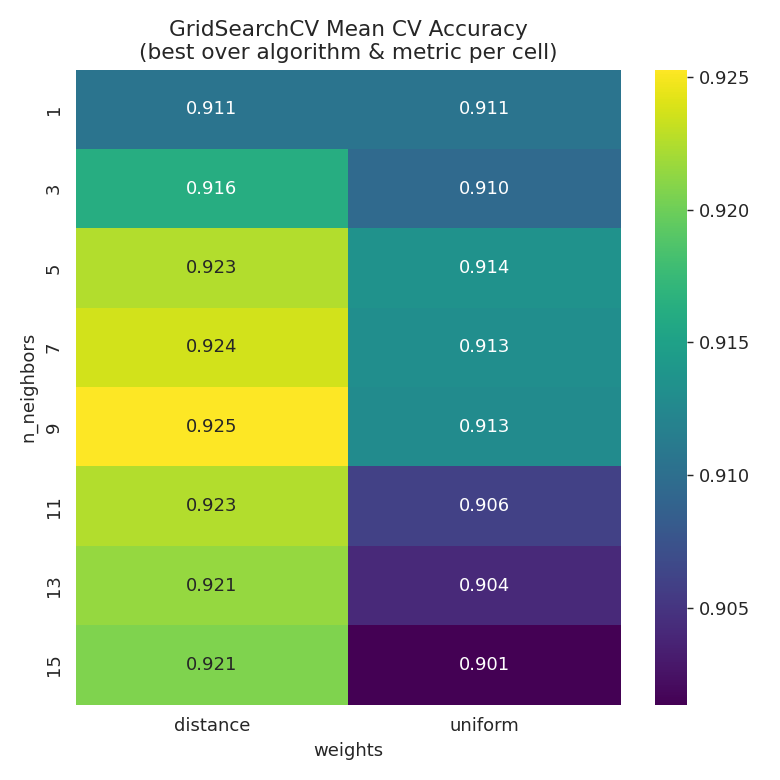
\includegraphics[width=0.55\linewidth]{figures/13_gridsearch_heatmap.png}
\caption{GridSearchCV mean cross-validation accuracy across $n\_neighbors$ and
$weights$ (best value over algorithm/metric shown per cell).}
\end{figure}
\textbf{Inference:} Distance-weighted KNN consistently outperforms uniform weighting at
every $k$, and accuracy peaks in the $k=7$--$11$ range before flattening, guiding the
search toward the reported optimum of $k=9$.

\begin{figure}[H]
\centering
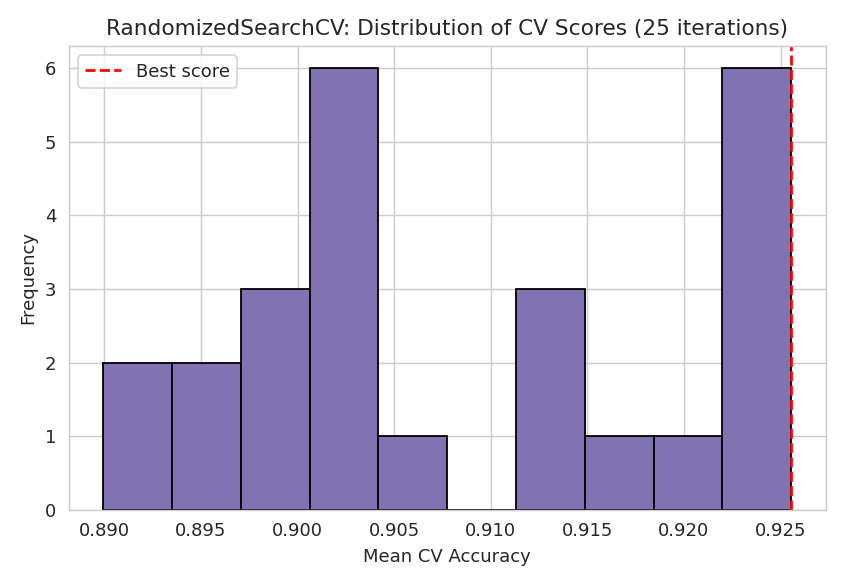
\includegraphics[width=0.6\linewidth]{figures/14_randomsearch_distribution.png}
\caption{Distribution of mean CV accuracy across the 25 RandomizedSearchCV iterations.}
\end{figure}
\textbf{Inference:} Most sampled configurations already achieve accuracy above 0.90,
and the best sampled score (0.9255) is statistically indistinguishable from the
exhaustive grid search optimum (0.9253), showing that random sampling of roughly 20\%
of the search space was sufficient to find a near-optimal configuration in less than
half the compute time.

\section{Discussion}

\subsection*{Analysis Questions}
\textbf{1. Which Na\"ive Bayes variant performed best?} Bernoulli NB, with the highest
accuracy (0.876), F1-score (0.837) and ROC-AUC (0.950) among the three variants. Its
binarize-then-model-presence/absence approach fits the heavily zero-inflated, right-skewed
nature of the Spambase features better than Gaussian NB's normality assumption or
Multinomial NB's pure count model.

\textbf{2. What is the optimal value of $k$?} Both search strategies converge to $k
\approx 8$--$9$ with distance-weighting and the Manhattan metric, achieving a 5-fold CV
accuracy of about 0.925, noticeably higher than the 0.910 obtained with the default
uniform-weight, Euclidean-distance configuration at the same $k$.

\textbf{3. Compare GridSearchCV and RandomizedSearchCV.} GridSearchCV exhaustively
evaluated all $8 \times 2 \times 2 \times 2 = 128$ combinations in 58.5 s and found a CV
accuracy of 0.9253. RandomizedSearchCV sampled only 25 combinations in 23.8 s (59\%
faster) and found a marginally higher score of 0.9255. For this search space the two
methods are effectively equivalent in quality, but RandomizedSearchCV is clearly more
time-efficient.

\textbf{4. Compare KDTree and BallTree.} Both produce identical predictions and
accuracy (they are exact, not approximate, neighbor searches), differing only in
construction/query speed. On this dataset BallTree built marginally faster (0.0115 s vs.
0.0167 s) and queried marginally faster (0.251 s vs. 0.266 s), though the difference is
small enough to be within run-to-run noise.

\textbf{5. Compare theoretical and practical complexity.} The measured times track the
theoretical expectations well: Naive Bayes trains and predicts in single-digit
milliseconds regardless of variant ($O(nd)$/$O(d)$), while KNN prediction (0.25--0.29 s)
is orders of magnitude slower than any NB variant, consistent with its $O(nd)$
brute-force / $O(\log n)_{avg}$ tree-based query cost. However, the tree-based speed-up
over brute force is muted here because $d=57$ is high enough that KDTree/BallTree
partitioning becomes less effective (the curse of dimensionality); both trees still
required a meaningful search rather than a near-$O(\log n)$ lookup.

\textbf{6. Which classifier is preferred for large datasets?} Na\"ive Bayes, because its
training and prediction costs scale linearly in $n$ and $d$ with very small constants
and no need to retain the full training set at inference time, whereas KNN's
prediction-time cost grows directly with the number of stored training points,
becoming a bottleneck as $n$ grows.

\subsection*{Additional Tasks}
\begin{itemize}
\item \textbf{Train-test split sensitivity:} Accuracy for both models was stable across
70/30, 80/20 and 90/10 splits (Bernoulli NB: 0.877--0.887; tuned KNN: 0.907--0.931),
indicating the results are not an artifact of one particular split. Both models perform
best with more training data relative to test data (70/30), as expected.
\item \textbf{Euclidean vs. Manhattan distance:} Manhattan distance gave higher
precision but lower recall than Euclidean at $k=9$; Euclidean gave the better overall
F1-score (0.883 vs 0.869) in the fixed-weights comparison, though the grid search found
that when combined with \emph{distance} weighting, Manhattan actually produced the best
overall configuration, showing that hyperparameters interact rather than acting
independently.
\item \textbf{Weighted KNN:} Distance-weighting improved accuracy, recall and F1-score
over uniform weighting at the same $k$, since it lets nearby neighbors dominate the vote
and reduces the influence of ties among more distant points.
\item \textbf{Overfitting/underfitting vs. $k$:} $k=1$ effectively memorizes the
training data (zero bias, high variance) and is the most overfit-prone setting, visible
here as the lowest test accuracy in the sweep. As $k$ increases to 7--11, variance drops
and accuracy improves; had $k$ been pushed much higher (e.g., $k \to n$), the decision
boundary would flatten toward predicting the majority class everywhere, causing
underfitting (rising bias). The plateau observed between $k=7$ and $k=11$ suggests this
dataset's sweet spot lies in that range.
\end{itemize}

\subsection*{Bias-Variance Trade-off}
Na\"ive Bayes classifiers are high-bias, low-variance models: their strong independence
assumption limits how well they can fit complex decision boundaries (visible in
Multinomial NB's comparatively low accuracy), but this same rigidity makes them stable
across resampling, as reflected in Bernoulli NB's tight cross-validation spread (std =
0.0147). KNN is a low-bias, higher-variance model whose flexibility (especially at small
$k$) lets it fit the training distribution closely, which is why tuning $k$ and the
weighting scheme had a measurable effect on its performance and why it ultimately
out-performed every Naive Bayes variant once properly tuned.

\section{Conclusion}
Both families of classifiers achieved strong performance on the Spambase dataset, but
with different trade-offs. Bernoulli Na\"ive Bayes was the best-performing and by far the
fastest of the Naive Bayes variants, thanks to its binarized, presence/absence modelling
of the skewed, zero-inflated feature set. The tuned KNN classifier ($k=9$,
distance-weighted, Manhattan distance) achieved the best overall accuracy (0.921) and
ROC-AUC (0.971) of all four models, at the cost of roughly two orders of magnitude
higher prediction latency. RandomizedSearchCV located an equally good configuration to
GridSearchCV in under half the time, making it the more practical choice for larger
hyperparameter spaces. For a production spam filter prioritizing throughput, Bernoulli
NB offers the best accuracy-per-millisecond; for a setting where prediction latency is
less critical than raw accuracy, the tuned KNN model is preferable.

\section{References}
\begin{enumerate}
\item F. Hopkins, E. Reeber, G. Forman, and J. Suermondt, ``Spambase Data Set,'' UCI
Machine Learning Repository, 1999. [Online]. Available:
\url{https://archive.ics.uci.edu/dataset/94/spambase}
\item Scikit-learn Developers, ``Naive Bayes,'' Scikit-learn Documentation. [Online].
Available: \url{https://scikit-learn.org/stable/modules/naive_bayes.html}
\item Scikit-learn Developers, ``Nearest Neighbors,'' Scikit-learn Documentation.
[Online]. Available: \url{https://scikit-learn.org/stable/modules/neighbors.html}
\item Scikit-learn Developers, ``Tuning the hyper-parameters of an estimator,''
Scikit-learn Documentation. [Online]. Available:
\url{https://scikit-learn.org/stable/modules/grid_search.html}
\item A. G\'eron, \textit{Hands-On Machine Learning with Scikit-Learn, Keras and
TensorFlow}, 3rd ed. Sebastopol, CA: O'Reilly Media, 2022.
\item C. M. Bishop, \textit{Pattern Recognition and Machine Learning}. New York:
Springer, 2006.
\end{enumerate}

\end{document}
